
\chapter{PROCESOS ESTOCÁSTICOS}

%Laura Morales Ariza
\newpage

En este capítulo se presentan los sistemas de ecuaciones lineales en diferencias estocásticos como modelos para describir las dinámicas internas y cruzadas entre las series de tiempo obtenidas del sistema dinámico $S$ en estudio. Aunque los modelos parten del supuesto de linealidad, las series
modeladas no tienen por qué serlo. Los mismos modelos incorporan mecanismos propios que permiten, a través de \textit{transformaciones}, estudiar y analizar conjuntos de series de tiempo que no presentan esta característica.

Existen otros tipos de modelos, tales como las redes neuronales artificiales (entre otros), que no suponen tal comportamiento lineal sobre los datos; sin embargo, ambos puntos de vista, el enfoque presentado aquí, usualmente conocido como \textit{análisis clásico de series de tiempo} y el \textit{análisis contemporáneo inspirado en el funcionamiento del cerebro humano} tienen ventajas y desventajas.
En tal virtud le corresponde al experto definir cuál de los dos debe emplear de acuerdo con la
situación particular.

El esquema y notación empleados en este documento están basados en  \cite{trivino2012esthocasticModels};\cite{wei1994timeseries}, en esos textos se detallan con mayor profundidad los resultados aquí presentados.


\section{INTRODUCCIÓN}\label{sec:intro1}
\setcounter{equation}{0}

Una \textit{serie de tiempo} es una secuencia ordenada de observaciones o, formalmente, una realización de
un proceso estocástico. Aunque el orden se hace usualmente a través del tiempo (en el sentido
cronológico), sobre todo en términos de algunos intervalos de tiempo equidistantes, el orden
también se puede tomar a través de otras dimensiones, como el espacio y más específicamente el
\textit{espacio-tiempo}. Las series de tiempo se producen en una variedad de campos. En la agricultura, se
observa precios diarios de cierre de acciones, tasas de interés, precios semanales índices mensuales,
las ventas trimestrales y ganancias anuales. En ingeniería, observamos sonido, señales eléctricas, y
el voltaje. En geofísica, registramos la turbulencia, como las olas del mar y el ruido de la tierra en un
área. En estudios médicos, medimos el trazado del electroencefalograma (EEG) y el
electrocardiograma (ECG). En meteorología, observamos velocidades por hora de viento,
temperatura diaria y las precipitaciones anuales. En el control de calidad, hacemos un seguimiento
de un proceso de acuerdo con un determinado valor objetivo. En ciencias sociales, se estudian las tasas anuales de natalidad, tasas de mortalidad, las tasas de accidentes, y varios índices de
criminalidad. La lista de las áreas en las que se observa la serie de tiempo y estudió es aún más
grande. En general, en el modelamiento de un sistema (complejo) $S$ concurren series de todas estas
disciplinas y, probablemente, muchas más; por ejemplo, índices de calidad de vida, series de tiempo
de impacto ambiental, datos cronológicos de catástrofes naturales, etc. Por tal razón se hace
necesario emplear instrumentos matemáticos apropiados que permitan describir la dinámica
subyacente en los datos como las relaciones entre las diferentes series y construir instrumentos que
permitan predecir valores o comportamientos futuros con unos niveles de error aceptados.\\


Hay diversos objetivos para el estudio de series de tiempo. Ellos incluyen la comprensión y
descripción del mecanismo de generación, la predicción o pronóstico de valores futuros, y un
control óptimo de sistema. La naturaleza intrínseca de una serie de tiempo es que sus observaciones
son dependientes o correlacionados, y el orden de las observaciones es por lo tanto importante. Por
lo tanto, los procedimientos estáticos y técnicas que se basan en hipótesis de independencia ya no
son aplicables, y, en consecuencia se hace necesario el empleo de otro tipo de métodos. El cuerpo de
la metodología estadística disponible para el análisis de series de tiempo se conoce como análisis de
series de tiempo. Y ese es el propósito de este documento, realizar un esbozo general pero no
profundo de tales técnicas.\\


En este capítulo, se presentan algunos conceptos fundamentales que son necesarios para la adecuada
comprensión de los modelos de series de tiempo que se incluyen en este documento. Las dinámicas
se describen a través de sistemas de ecuaciones en diferencias estocásticas lineales homogéneas con
coeficientes constantes. Se presentan las funciones de autocorrelación y autocorrelación parcial y la
noción de ruido blanco, y también los estimadores de la media, la autocovarianza y la correlación.
Con base en esas estimaciones se describe el método de identificación de los modelos.

\section{ECUACIONES EN DIFERENCIAS LINEALES HOMOGÉNEAS}\label{sec:ecuac} 

\subsection{Operador de retardo y de diferencias}

Dada una serie $X_{t}$, el operador de retardo $B$, que se ilustra en la Figura \arabic{chapter}.1, atrasa en una unidad
la serie de tiempo, es decir $X_{t-1} = BX_{t}$. Este operador puede generalizarse para que desfase la serie $k$ unidades de tiempo. Este hecho se escribe formalmente como $X_{t-k} = B^{k} X_{t}$ y se representa esquemáticamente en la Figura \arabic{chapter}.2.

\begin{figure}[H]
     \begin{center}
         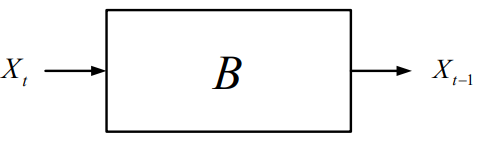
\includegraphics[width=100mm]{chapters/chapter2/figures/operadorretardo.PNG}
     \end{center}
     \textbf{\caption{Operador de retardo}}
     \label{fig:1}
\end{figure}

\begin{figure}[H]
     \begin{center}
         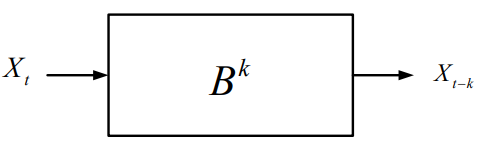
\includegraphics[width=100mm]{chapters/chapter2/figures/operadorretardotiempo.PNG}
     \end{center}
     \textbf{\caption{Operador de retardo de k unidades de tiempo}}
\end{figure}

De forma similar el operador de diferencias trabaja de la forma descrita en la Figura \arabic{chapter}.3, es decir, dada la serie $\dot{X}_{t}$ su \textit{d ésima} diferencia está dada por $X_{t} = (1-B)^d$ $\dot{X}_{t} = \sum_{k=0}^d {d \choose k} (-1)^{d-k} \dot{X}_{d-k}$.

\begin{figure}[H]
     \begin{center}
         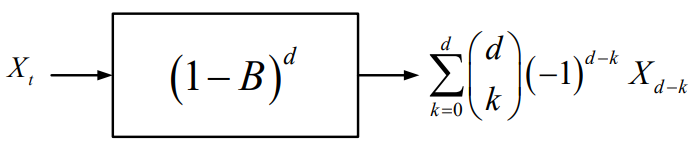
\includegraphics[width=120mm]{chapters/chapter2/figures/operadordiferencias.PNG}
     \end{center}
     \textbf{\caption{Operador de diferencias}}
\end{figure}

\subsection{Solución general de una ecuación en diferencias lineal homogénea}

****No hay contenido *****

\section{PROCESOS ESTOCÁSTICOS Y SERIES DE TIEMPO}\label{sec:procestoc}

Un proceso estocástico se define matemáticamente como un conjunto de variables aleatorias $\{X_{t_{i}}\}^{i=n}_{i=1}$ que siguen la distribución conjunta de la ecuación \ref{onePoint} donde $\{x_{i}\}^{i=n}_{i=1} \in \mathbb{R}^n$.

\begin{equation}
F_{X_{t_{1}},X_{t_{2}},...,X_{t_{n}},} (X_{1},X_{2},...,X_{n}) = P[w: X_{t_{1}} \leq x_{1},X_{t_{2}} \leq x_{2},...,X_{t_{n}} \leq x_{n}]
\label{onePoint}
\end{equation}
\\

Por su parte una serie de tiempo es una realización de un proceso estocástico. Es decir, es un
conjunto de valores $\{x_{i}\}^{i=n}_{i=1} \in \mathbb{R}^n$ que han sido tomados de la distribución conjunta (\ref{onePoint}).

Por ejemplo, como resultado del proceso de simulación en el prototipo del sistema en estudio $S$ se obtienen decenas de tablas con series de tiempo similares a las presentadas en la Figura \arabic{chapter}.4 (donde
solamente aparecen dos tablas). Esos datos pueden ser representados en un sistema cartesiano como
el de la Figura \arabic{chapter}.5.

\begin{figure}[H]
     \begin{center}
         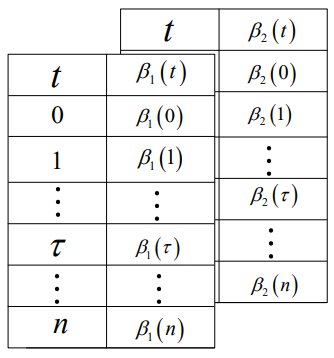
\includegraphics[width=70mm]{chapters/chapter2/figures/dosseriestiempo.PNG}
     \end{center}
     \textbf{\caption{Dos series de tiempo de dos indicadores en el sistema $S$}}
\end{figure}

\begin{figure}[H]
     \begin{center}
         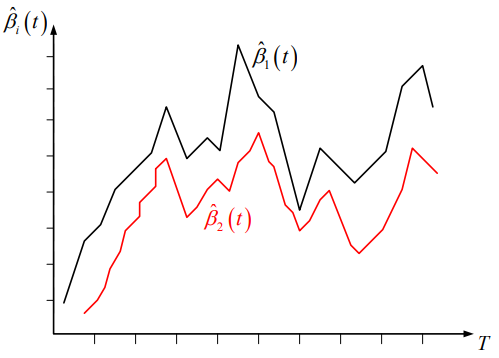
\includegraphics[width=100mm]{chapters/chapter2/figures/mateseriestiempo.PNG}
     \end{center}
     \textbf{\caption{Representación matemática de las series de tiempo de dos indicadores}}
\end{figure}

\section{FUNCIONES DE AUTOCOVARIANZA, AUTOCORRELACIÓN Y AUTOCORRELACIÓN PARCIAL}\label{sec:autovar}

\subsection{Definiciones formales}

Para un proceso estacionario $\{X_{t}\}^{t=n}_{t=1}$, la media $E(X_{t}) = \mu_{X}$ y la varianza $\sigma^{2}_{X} = Var(X_{t}) = E(X_{t}-\mu_{X})^2 $ son constantes, y las covarianzas $Cov(X_{t},X_{s})$, son funciones
únicamente de la diferencia de tiempo $k=|t-s|$. Por lo tanto, en este caso, se describe la covarianza
entre $X_{t}$ y $X_{t+k}$ de acuerdo con la ecuación (\ref{twoPoint}).

\begin{equation}
\gamma_{k} = Cov(X_{t},X_{s}) =  E(X_{t}-\mu_{X})(X_{t+k}-\mu_{X})
\label{twoPoint}
\end{equation}
\\

Y la correlación entre $X_{t}$ y $X_{t+k}$ como se presenta en la ecuación (\ref{threePoint}).

\begin{equation}
\rho_{k} = \frac{Cov(X_{t},X_{t+k})}{\sqrt{Var(X_{t})} \sqrt{Var(X_{t+k})}} = \frac{\gamma_{k}}{\gamma_{0}}
\label{threePoint}
\end{equation}
\\

donde $\sigma^{2}_{X} = Var(X_{t}) = Var(X_{t+k}) = \gamma_{0}$. Como funciones de $k$, $\gamma_{k}$ se denomina función de autocovarianza y $\rho_{k}$ se llama función de autocorrelación (ACF) en el análisis de series de tiempo, ya que representan la covarianza y la correlación entre $X_t$ y $X_{t+k}$ desde el mismo proceso, separadas únicamente por $k$ unidades de tiempo. Una función de autocorrelacion típica se presenta en la Figura \arabic{chapter}.6.

Además de la autocorrelación entre $X_t$ y $X_{t+k}$, se requiere conocer la correlación entre $X_t$ y $X_{t+k}$ dado que se conocen los valores de las variables aleatorias $X_{t+1},X_{t+2},...,$ y $X_{t+k-1}$. En términos
matemáticos esto se expresa mediante la ecuación (\ref{fourPoint}).

\begin{equation}
\phi_{kk} = Corr(Z_t,Z_{t+k}|Z_{t+1},...,Z_{t+k-1})
\label{fourPoint}
\end{equation}
\\

\begin{figure}[H]
     \begin{center}
         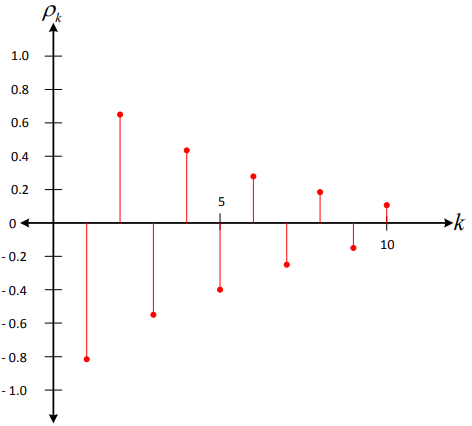
\includegraphics[width=90mm]{chapters/chapter2/figures/fautocorrelacion.PNG}
     \end{center}
     \textbf{\caption{Una función de autocorrelación típica}}
\end{figure}


La expresión (\ref{fourPoint}) se refiere generalmente como la autocorrelación parcial en el análisis de series
de tiempo. Puede demostrarse que la expresión (\ref{fourPoint}) es equivalente a la ecuación (\ref{fivePoint}).

\begin{equation}
\phi_{11} = \rho_{1}
\label{fivePoint}
\end{equation}
\\

\begin{equation*}
\phi_{kk} =  \frac{
\left| 
\begin{array}{cccccc}
1 & \rho_{1} & \rho_{2} & \cdots & \rho_{k-2} & \rho_{1} \\
\rho_{1} & 1 & \rho_{1} & \cdots & \rho_{k-3} & \rho_{2} \\
\vdots & \vdots & \vdots & \ddots & \vdots & \vdots\\
\rho_{k-1} & \rho_{k-2} & \rho_{k-3} & \cdots & \rho_{1} & \rho_{k} \\
\end{array}
\right|}{
\left| 
\begin{array}{cccccc}
1 & \rho_{1} & \rho_{2} & \cdots & \rho_{k-2} & \rho_{k-1} \\
\rho_{1} & 1 & \rho_{1} & \cdots & \rho_{k-3} & \rho_{k-2} \\
\vdots & \vdots & \vdots & \ddots & \vdots & \vdots\\
\rho_{k-1} & \rho_{k-2} & \rho_{k-3} & \cdots & \rho_{1} & 1 \\
\end{array}
\right|
} 
\end{equation*}
\\

\chapter{SERIES DE TIEMPO}
\chapter{CADENAS DE MARKOV}

